\chapter{Interpretazione astratta}

L'interpretazione astratta è una tecnica di analisi statica che consiste nel definire un approssimazione \emph{corretta} e \emph{decidibile} della semantica del programma da analizzare \cite{cousot}.

\section{Semantica}

\begin{definition}[Semantica]
La semantica di un programma $P$ è la descrizione formale di come il programma viene eseguito. Si denota con $\semantics{P}$. 
\end{definition}

I programmi scritti in linguaggi imperativi sono composti da istruzioni che vengono eseguite in sequenza. Ad ogni passo di computazione, la macchina aggiorna una tabella detta \emph{memoria} di associazioni variabile$\rightarrow$valore. La semantica che descrive i programmi dovrà formalizzare il concetto di \emph{esecuzione di una istruzione}. 

Una rappresentazione efficace è quella del \emph{control flow graph}. Il control flow graph è un grafo $\struct{V, E \subseteq V \times V}$ tale che l'insieme $V = \set{Point}$ dei vertici sono i punti del programma e l'insieme $E$ degli archi è l'insieme delle istruzioni. 

\subsection{Trace semantics}

\begin{definition}[Sistema di transizioni (parzialmente preso da {\cite[p.~88]{mastro16}})]
Un \emph{sistema di transizioni} è una struttura $\struct{\mathbf{S}, \to}$ del programma $P$ dove $\mathbf{S}$ è un insieme di stati (``fotografie" della memoria in un certo istante) ed $\to$ è una relazione binaria tra stati tale che
\[ \sigma \to \sigma' \iff \sigma' \text{ è un possibile successore di } \sigma; \quad \sigma, \sigma' \in \mathbf{S} \]
\end{definition}

La relazione $\to$ formalizza il concetto di passo di esecuzione. Una sequenza di stati $\sigma_0 \sigma_1 ... \sigma_n$ è detta \emph{trace}. Ogni trace rappresenta una esecuzione di un programma è può anche essere infinita. Da questa si può definire la \emph{trace semantics} (per approfondimenti vedi \cite{xavier}).

Guardando la trace semantics possiamo verificare se, per una certa trace ed in un certo punto dell'esecuzione, vale la proprietà da verificare.

Dato un sistema di transizioni $\struct{\mathbf{S}, \to}$ del programma $P$ la \emph{trace semantics} $\semantics{\mathbf{S}}$ è l'insieme delle possibili tracce di esecuzione di $P$:
\[ \semantics{\mathbf{S}} = \{ \sigma_0 \sigma_1 ... \sigma_n \mid \forall i \;\, \sigma_i \in \mathbf{S} \land (\sigma_i \to \sigma_{i+1}) \} \]

Questo tipo di semantica ci lega alle informazioni temporali tipiche di una trace: in un certo momento la proprietà da verificare può valere mentre in un altro no. Preferiremmo semplificare il processo e considerare solo le proprietà \emph{invarianti}, che valgono per ogni trace: utilizziamo la \emph{collecting semantics}.

\subsection{Collecting semantics}

La collecting semantics di un programma $P$ rappresentato dal control flow graph $\struct{\set{Point}, E}$ è una funzione
\[ \mathcal{C\!\!S} : \set{Point} \to \wp(\set{State}) \]
che associa ad un punto del programma l'insieme dei possibili stati che può avere. Conoscendo la collecting semantics di $P$ possiamo facilmente verificare se la nostra proprietà vale o meno. $\mathcal{C\!\!S}$ può essere ricavata tramite un algoritmo di fixpoint iterativo (per approfondire vedi Sezione~\ref{sec:fixpoint}). 

\begin{example}\label{example:collecting}
Calcola la collecting semantics del seguente pezzo di codice.
\begin{javascriptcode}
x = 0;
y = 2;
while (x < 3) {
    y = y * y;
    x = x + 1;
}
\end{javascriptcode}
Lo stato che dobbiamo mantenere è una coppia $\struct{x,y}$ che all'inizio ha valore $\set{INIT} = \{ \struct{0, 2} \}$. La funzione di cui dobbiamo trovare il least fix-point è
\[ P(M) = \texttt{WHILE}_{x<3}(\texttt{INCX}(\texttt{SQUAREY}(M)), \set{INIT}) \]
con 
\begin{align*}
    \texttt{SQUAREY}(M) &= \{ \struct{x,y^2} \mid \struct{x,y} \in M \} \\
    \texttt{INCX}(M) &= \{ \struct{x+1,y} \mid \struct{x,y} \in M \} \\
    \texttt{WHILE}_{x<3}(M, I) &= (M \cup I) \cap \{ \struct{x,y} \mid x < 3 \} 
\end{align*}

Procediamo col metodo iterativo:
\begin{align*}
    P(\varnothing) 
        &= (\texttt{INCX}(\texttt{SQUAREY}(\varnothing)) 
        \cup \{ \struct{0, 2} \} ) 
        \cap \{ \struct{x,y} \mid x < 3 \} \\
        &= \{ \struct{0, 2} \} \\
    P(\{ \struct{0, 2} \}) 
        &= (\texttt{INCX}(\texttt{SQUAREY}(\{ \struct{0, 2} \})) \\
        &\hphantom{=} \cup \{ \struct{0, 2} \} ) 
        \cap \{ \struct{x,y} \mid x < 3 \} \\
        &= \{ \struct{0, 2},  \struct{1, 4} \} \\
    P(\{ \struct{0, 2},  \struct{1, 4} \}) 
        &= (\texttt{INCX}(\texttt{SQUAREY}(\{ \struct{0, 2},  \struct{1, 4} \})) \\
        &\hphantom{=} \cup \{ \struct{0, 2} \} ) 
        \cap \{ \struct{x,y} \mid x < 3 \} \\
        &= \{ \struct{0, 2},  \struct{1, 4}, \struct{2, 16} \} \\
    P(\{ \struct{0, 2},  \struct{1, 4}, \struct{2, 16} \} ) 
        &= (\texttt{INCX}(\texttt{SQUAREY}(\struct{0, 2},  \struct{1, 4}, \struct{2, 16})) \\
        &\hphantom{=} \cup \{ \struct{0, 2} \} ) 
        \cap \{ \struct{x,y} \mid x < 3 \} \\
        &= \{ \struct{0, 2},  \struct{1, 4}, \struct{2, 16}, \struct{3, 64} \}
        \cap \{ \struct{x,y} \mid x < 3 \} \\
        &= \{ \struct{0, 2},  \struct{1, 4}, \struct{2, 16} \}
\end{align*}

Il least fix-point è il valore di memoria $M = \{ \struct{0, 2},  \struct{1, 4}, \struct{2, 16} \}$.
\end{example}

La semantica collecting è in generale indecidibile. Occorre trovare un modo per renderla decidibile: utilizziamo i \emph{domini astratti}.





\newcommand{\uco}{\fun{uco}}
\newcommand{\lfp}{\fun{lfp}}

\section{Teoria dei reticoli}

\subsection{Poset}

\begin{definition}[Poset (parzialmente preso da \cite{mastro16})]
Un \emph{insieme parzialmente ordinato} o \emph{poset} è una struttura $\struct{P, \sqsubseteq}$ tale che $P$ è un insieme e $\sqsubseteq$ è una relazione binaria su $P$ che gode di proprietà \emph{riflessiva}, \emph{antisimmetrica} e \emph{transitiva}. 
\end{definition}

In una relazione d'ordine parziale $\sqsubseteq$ non è detto che tra due elementi $x,y \in P$ questi siano confrontabili, cioè che valga $x \sqsubseteq y \lor y \sqsubseteq x$. In questo caso si scrive $x || y$. Se tutti gli elementi dell'insieme sono a due a due confrontabili, la relazione d'ordine si dice \emph{totale} e viene indicata col simbolo $\le$. 

Esempi di poset le strutture $\struct{\mathbb{Z}, \le}$ (che è anche un insieme totalmente ordinato), la struttura $\struct{\wp(S), \subseteq}$ formata dall'insieme delle parti di un insieme $S$ e la relazione di inclusione insiemistica (Figura~\ref{fig:poset-parti}), ma anche la struttura $\struct{\{1,2,3,4,6,12\}, \mathbf{divide}}$.

\begin{figure}[htbp]
    \centering
    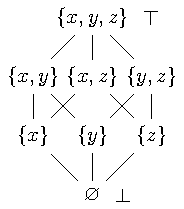
\includegraphics{capitoli/interpretazione-astratta/immagini/poset-parti.pdf}
    \caption{Poset $\struct{\wp(S), \subseteq}$ con $S = \{x,y,z\}$}
    \label{fig:poset-parti}
\end{figure}

\begin{definition}[Elementi top e bottom (parzialmente preso da \cite{mastro16})]
All'interno di un poset $\struct{P, \sqsubseteq}$ si può individuare, se esiste, l'elemento top $\top \in P$ tale che $\forall x \in P . x \le \top$. Se l'elemento $\top$ esiste, è unico. L'elemento bottom $\bot$ è definito in modo duale.
\end{definition}

All'interno del poset $\struct{\wp(S), \subseteq}$ l'elemento top è $\top = S$ e il bottom è $\bot = \varnothing$. All'interno del poset $\struct{\mathbb{Z}, \le}$ non esiste l'elemento top ma esiste l'elemento bottom $\bot = 0$. Se ad $\mathbb{Z}$ aggiungiamo un ulteriore elemento $\infty$ tale che $\forall n \in \mathbb{Z} . n < \infty$ allora questo elemento funge da top per la nuova struttura $\struct{\mathbb{Z} \cup \{ \infty \}, \le}$ creata.

\begin{definition}[Least upper bound (parzialmente preso da \cite{mastro16})]
L'operazione di \emph{least upper bound} (o \emph{lub}, \emph{join}, \emph{estremo superiore}) tra due elementi $x,y \in P$ di un poset $\struct{P, \sqsubseteq}$ se esiste è l'elemento $\join[x][y] = z \in P$ tale che:
\begin{itemize}
    \item $\join[x][y]$ è maggiorante di $x$ e $y$ ($x,y \sqsubseteq \join[x][y]$);
    \item $\join[x][y]$ è il più piccolo maggiorante di $x$ e $y$ ($\forall m \in P . (x,y \sqsubseteq m \to \join[x][y] \sqsubseteq m)$);
    \item $\join[x][y]$ è unico.
\end{itemize}
\end{definition}

\begin{definition}[Greatest lower bound (parzialmente preso da \cite{mastro16})]
L'operazione di \emph{greatest lower bound} (o \emph{glb}, \emph{meet}, \emph{estremo inferiore}) è definito in modo duale al lub e di indica con $\meet[x][y]$ per $x,y \in P$.
\end{definition}

Il join (e il meet) di due elementi del poset può non essere definito per due motivi: \emph{l'elemento manca} (in $\struct{\{1,2,3,4,6,12,13\}, \mathbf{divide}}$ l'elemento $\join[12][13]$ non è definito poichè non c'è elemento maggiorante di entrambi) oppure \emph{non è rispettata la condizione di unicità} (se ci sono più maggioranti non confrontabili tra loro).

\begin{definition}[Catena (parzialmente preso da \cite{mastro16})]
Un sottoinsieme $C \subseteq P$ del poset $\struct{P, \sqsubseteq}$ è detto \emph{catena} se gli elementi di $C$ sono a due a due confrontabili tra loro. Il duale della catena è l'anticatena (elementi non confrontabili tra loro).  
\end{definition}

\begin{definition}[Condizione ACC (parzialmente preso da \cite{mastro16})]
Una catena $C$ soddisfa la \emph{ascending chain condition} se $C$ è un insieme finito oppure se da un certo $n$ in poi si ha $\forall m > n . c_n = c_m$.
\end{definition}

\begin{definition}[Poset completo (parzialmente preso da \cite{mastro16})]
Un poset $\struct{P, \sqsubseteq}$ si dice completo (abbreviato \emph{c.p.o.}) se per ogni sua catena $C$ anche infinita esiste l'estremo superiore $\join[C] \in P$.
\end{definition}

\subsection{Reticoli}\label{sec:reticoli}

\begin{definition}[Reticolo (parzialmente preso da \cite{mastro16})]
Un reticolo è una struttura $\struct{P, \sqsubseteq, \join, \meet}$ nella quale $\struct{P, \sqsubseteq}$ è un poset, l'operazione binaria $\join$ effettua il lub, l'operazione $\meet$ effettua il glb ed 
\[ \forall x,y \in P \text{ sono definiti } \join[x][y], \meet[x][y] \in P \]
\end{definition}

\begin{definition}[Sottoreticolo (parzialmente preso da \cite{mastro16})]
Un sottoinsieme $Q \subseteq P$ del reticolo $\struct{P, \sqsubseteq, \join, \meet}$ è detto \emph{sottoreticolo} se $Q$ è chiuso per lub e glb ($\forall x,y \in Q . \join[x][y], \meet[x][y] \in Q$). 
\end{definition}

\begin{definition}[Reticolo completo (parzialmente preso da \cite{mastro16})]
Un reticolo che è anche c.p.o. viene detto reticolo completo.
\end{definition}

\subsection{Ordinamento pointwise di funzioni}

Date due funzioni $f_1, f_2 : C \to C$, il loro ordinamento parziale $\le$ è detto \emph{pointwise}, e si scrive $f_1 \le f_2$, se
\[ \forall x \in C \left[ f_1(x) \le f_2(x) \right] \]

\subsection{Connessione di Galois}\label{sec:galois}

\begin{definition}[Connessione di Galois]
Dati due poset $\struct{C, \le}$ e $\struct{A, \preceq}$, la coppia di funzioni $\struct{\alpha, \gamma}$ viene definita \emph{connessione di Galois} e si indica con 
\[ C \galois{\alpha}{\gamma} A \]
dove
\begin{itemize}
    \item[$C$:] insieme detto dominio concreto;
    \item[$\gamma$:] funzione monotona di concretizzazione $\gamma : A \to C$, $\forall c \in C : c \le \gamma(\alpha(c))$;
    \item[$A$:] insieme detto dominio astratto;
    \item[$\alpha$:] funzione monotona di astrazione $\alpha : C \to A$, $\forall a \in A : a \preceq \alpha(\gamma(a))$.
\end{itemize}
\end{definition}

\begin{definition}[Connessione di Galois come adjunctor (parzialmente preso da \cite{mastro16})]
La struttura è detta anche \emph{adjunctor} ($\alpha$ left adjoint, $\gamma$ right adjoint) poichè vale che
$$\forall c \in C, a \in A \; : \; \alpha(c) \preceq a \Leftrightarrow c \le \gamma(a)$$
\end{definition}

\begin{definition}[Connessione di Galois come funzioni additive e co-additive (parzialmente preso da \cite{mastro16})]
In una connessione di Galois la funzione $\alpha$ è additiva, cioè preserva l'operazione di join: 
$$\alpha\left(\join[X]\right) = \join[\alpha(X)] \text{ per ogni } X \subseteq C$$
e la funzione $\gamma$ è co-additiva, cioè preserva l'operazione di meet.
\end{definition}

\begin{definition}[Inserzione di Galois (parzialmente preso da \cite{mastro16})]
Una connessione di Galois si dice \emph{inserzione di Galois} e si scrive $C \galoiS{\alpha}{\gamma} A$ se $\alpha \circ \gamma = \fun{id}$. Sono equivalenti le seguenti espressioni:
\begin{itemize}
    \item $C \galoiS{\alpha}{\gamma} A$;
    \item $\alpha$ è suriettiva;
    \item $\gamma$ è iniettiva.
\end{itemize}
\end{definition}

Le inserzioni di Galois sono molto simili alle connessioni. La differenza tra i due è che nelle connessioni è possibile che più elementi del dominio astratto corrispondano allo stesso elemento del dominio concreto. Togliendo questi elementi ``superflui" si ottiene una inserzione. Questo procedimento, detto \emph{reduction} è sempre possibile e consiste nell'identificare in una classe di equivalenza gli elementi del dominio astratto con la stessa concretizzazione.

\subsection{Closure operators}

Un'interpretazione astratta può essere definita equivalentemente come una inserzione di Galois oppure come un operatore di chiusura.

\begin{definition}[Upper closure operator (da \cite{ranzato})]
Una funzione $\rho: L \to L$ è detta \emph{upper closure operator} se
\begin{enumerate}
    \item monotona: $x \le y \to \rho(x) \le \rho(y)$;
    \item estensiva: $x \le \rho(x)$;
    \item idempotente: $\rho(\rho(x)) = \rho(x)$.
\end{enumerate}
\end{definition}

Dato un reticolo completo $C$, un'operatore di chiusura $\rho$ è determinato univocamente dalla sua immagine $\rho(C) = \mathrm{codomain}(\rho)$. L'immagine di un $\rho$ coincide con l'insieme dei suoi \emph{fixpoint}:
\[ \rho(y) = \meet[\{x \mid x \in \mathrm{codomain}(\rho) \land y \le x \}] \]

\begin{definition}[Famiglia di Moore (da \cite{ranzato})]
Un sottoinsieme $X \subseteq L$ di un reticolo completo $L$ è detto \emph{famiglia di Moore} se $X$ è chiuso rispetto all'operazione di \emph{meet}, cioè
$$X = \mathcal{M}(X); \qquad \mathcal{M}(X) = \Big\{ \meet[S] \; \big| \; S \subseteq X \Big\}$$
\end{definition}

Viceversa, un'operatore $\rho$ sul dominio $J$ è un $\uco$ se e solo se il suo codominio $\rho(J) = K$ è una famiglia di Moore ed in quel caso $\rho(y) = \meet[\{x \mid x \in K \land y \le x \}]$. 

\subsection{Reticolo delle interpretazioni astratte}

Se $C$ è un reticolo completo, allora $\uco(C)$ forma un reticolo completo rispetto all'ordinamento pointwise con elemento $\top = \lambda x . \top$ e $\bot = \lambda x . x$. 

Dato $\rho \in \uco(C)$ ed un dominio astratto $A$, se $\rho(C)$ è isomorfico ad $A$ abbiamo $\iota: \rho(C) \to A$ ed $\iota^{-1} : A \to \rho(C)$. Allora la struttura
\[ \struct{\iota \circ \rho, C, A, \iota^{-1}} \]
è un'inserzione di Galois. Allo stesso tempo se $\struct{\gamma, C, A, \alpha}$ è un'inserzione di Galois allora $\rho_{A} = \gamma \circ \alpha$ è un $\uco(C)$.  

Definiamo l'insieme $\mathrm{Abs}(C)$ come l'insieme dei domini astratti di $C$. L'insieme forma un reticolo completo rispetto all'operazione di ordinamento
\[ A_1 \sqsubseteq A_2 
\iff \rho_{A_1} \subseteq \rho_{A_2} 
\iff \left( 
    \forall x . \rho_{A_1}(x) \le \rho_{A_2}(x)
\right) \]
e nel caso si dice che $A_1$ è più preciso (o più concreto) di $A_2$. La struttura $\struct{\mathrm{Abs}(C), \sqsubseteq}$ forma un reticolo completo detto \emph{reticolo delle interpretazioni astratte} ed è isomorfico al reticolo $\struct{\uco(C), \sqsubseteq}$. 

\subsection{Fixpoint}\label{sec:fixpoint}

\begin{definition}[Fixpoint (da \cite{mastro16})]
Data $f:X \to X$, il punto $x \in X$ si definisce fixpoint se $f(x) = x$.
\end{definition}

\begin{definition}[Least fixed point (da \cite{mastro16})]
Data $f:X \to X$, il punto $\lfp(f) = x \in X$ si definisce \emph{least fixed point} se per ogni $y$ fixpoint si ha $x \le y \to x = y$.
\end{definition}

\begin{theorem}[Teorema di Knaster-Tarski (da \cite{mastro16})]
Data una funzione $f:L \to L$ monotona su un reticolo completo $\struct{L, \le}$ esiste un unico $\lfp(f)$.
\end{theorem}

E' possibile calcolare $\lfp(f)$ tramite il metodo iterativo:
$$\bot \le f(\bot) \le f^2(\bot) \le ... \le f^n(\bot) = \lfp(f) = f^{n+1}(\bot) = f^{n+2}(\bot) = ...$$

\subsection{Widening}

I domini concreti $C$ possono avere infiniti valori. I domini astratti che abbiamo visto possono avere valori finiti (dominio dei segni) o infiniti (dominio degli intervalli). A volte non è possibile garantire la convergenza dei calcoli su domini infiniti (non rispettando la condizione di ACC). Si definisce allora una funzione detta widening che garantisce la terminazione a costo di perdere ulteriore precisione.

\begin{definition}[Widening binario (da \cite{mastro16})]
L'operatore di widening $\wide: P \times P \to P$ su un poset $\struct{P, \le}$ soddisfa le seguenti condizioni:
\begin{itemize}
    \item $\forall x,y \in P \, . \, x \le (\wide[x][y]) \land y \le (\wide[x][y])$;
    \item Per ogni catena $x_0 \le x_1 \le ...$ si definisce la catena \emph{non strettamente crescente} $y_0 = x_0, ..., y^{n+1} = \wide[x][y^n]$.
\end{itemize}
\end{definition}

L'operatore di widening non è commutativo ne associativo. L'iterazione col widening si svolge come segue:
$$x^0 = \bot \qquad x^{n+1} = \begin{cases} 
    x^n,                & f(x^n) \le x^n \\ 
    \wide[x^n][f(x^n)], & f(x^n) \not\le x^n \\
\end{cases}$$

\section{Dominio astratto}

Nell'Esempio~\ref{example:collecting}, la computazione del least fiexed point può diventare molto costosa: gli elementi dell'insieme $M$ sono coppie di tipo $\Z \times \Z$ e il loro numero può velocemente esplodere. Cerchiamo un modo per approssimare $M$. 

\begin{definition}[Dominio]
Il \emph{dominio} è l'insieme dei valori che le variabili possono assumere all'interno dello store. 
\end{definition}

Al posto che mantenere di ogni valore il numero esatto $n \in \Z$, ne manteniamo solamente la parte di informazione che ci interessa.

\begin{example}\label{example:sign}
Il dominio dei segni è definito come segue:
\[ \set{Sign} = \{ \top, \oplus, \ominus, 0, \bot \} \]
dove $\top$ rappresenta un qualsiasi numero, $\oplus$ i numeri positivi o o nulli, $\ominus$ quelli negativi o nulli, $0$ il sono numero zero e $\bot$ nessun numero (usato come condizione d'errore, per esempio la divisione per zero). 
\end{example}

\begin{example}\label{example:interval}
Il dominio degli intervalli è definito come segue:
\[ \set{Interval} = \{ [l,h] \mid l,h \in \Z; \; l \le h \} \]
\end{example}

Entrambi i domini in Esempio~\ref{example:sign} e Esempio~\ref{example:interval} sono approssimazioni del dominio $\wp(\Z)$. I primi due prendono il nome di \emph{dominio astratto} mentre quest'ultimo è detto \emph{dominio concreto}. I domini devono formare una struttura di reticolo completo (per approfondire vedi Sezione~\ref{sec:reticoli}).

\subsection{Connessioni di Galois}\label{sec:galois-c}

Uno dei costrutti matematici che mette in relazione il dominio concreto con quello astratto è la \emph{connessione di Galois} (vedi \ref{sec:galois}). Attraverso la coppia di funzioni $\alpha, \gamma$ mappiamo gli elementi del dominio concreto in quello astratto e viceversa. 

\begin{example}
Per il dominio di Esempio~\ref{example:sign}, le funzioni $\alpha$ e $\gamma$ sono definite come segue:
\begin{align*}
    \alpha(\varnothing)                                   & = \bot                 &
    \gamma(\bot)                                          & = \varnothing          \\
    \alpha(\{0\})                                         & = 0                    &
    \gamma(0)                                             & = \{ 0 \}              \\
    \alpha(\{ x \mid \min x \ge 0 \}) & = \oplus          &
    \gamma(\oplus)                                        & = \{ x \mid x \ge 0 \} \\
    \alpha(\{ x \mid \max x \le 0 \}) & = \ominus         &
    \gamma(\ominus)                                       & = \{ x \mid x \le 0 \} \\
    \alpha(\{ x \mid \min x < 0 \land \max x > 0\})       & = \top                 &
    \gamma(\top)                                          & = \mathbb{Z}
\end{align*}
\end{example}

\begin{figure}[htbp]
    \centering
    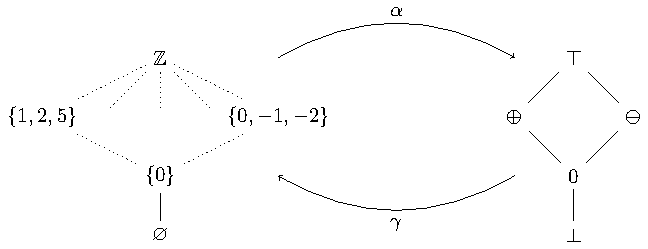
\includegraphics{capitoli/interpretazione-astratta/immagini/reticolo-segni.pdf}
    \caption{Connessione di Galois}
    \label{fig:galois-Z-sign}
\end{figure}

\subsection{Operazioni astratte}

Una volta definito il dominio astratto e la connessione di Galois, per ogni operazione $f : C \to C$ nel dominio concreto dobbiamo definire l'operazione $f^{\#} : A \to A$ nel dominio astratto. Il modo più immediato di definire $f^{\#}$ è tramite la \emph{best correct approximation}.

\begin{definition}[Best correct approximation (parzialmente preso da \cite{ranzato})]
Data una funzione $f : C \to C$ e una connessione di Galois $C \galois{\gamma}{\alpha} A$, si definisce $f^{\#} = \alpha \circ f \circ \gamma$ la \emph{best correct approximation} di $f$ in $A$.
\end{definition}

Tuttavia vorremmo poter avere il risultato di $f^{\#}$ senza dover eseguire $f$, in quanto questa potrebbe non essere calcolabile. Possiamo definire in un altro modo $f^{\#}$ e poi dimostrarne la correttezza.

\begin{definition}[Correttezza di una funzione astratta (parzialmente preso da \cite{ranzato})]
Data la connessione di Galois $C \galois{\gamma}{\alpha} A$ tra i due poset $\struct{C, \le}$ e $\struct{A, \preceq}$ ed una funzione concreta $f$, la funzione astratta $f^{\#}$ è un'approssimazione corretta di $f$ se vale
\[ \alpha \circ f = f^{\#} \circ \alpha \]
o equivalentemente
\[ f \circ \gamma = \gamma \circ f^{\#} \]
\end{definition}

\begin{example}
Consideriamo la funzione concreta $\fun{add} : \wp(\Z) \times \wp(\Z) \to \wp(Z)$:
\[ \fun{add}(X, Y) = \{ x + y \mid \forall x \in X, \, y \in Y \} \]
Per definire la sua funzione astratta nel dominio dei segni abbiamo più possibilità:
\begin{align*}
    \fun{add}^{\#}_1(s, t) 
    & = \alpha\big(\fun{add}(\gamma(s), \gamma(t)) \big) \\[1em]
    \fun{add}^{\#}_2(s,t) 
    & = \begin{array}{c c c c c c}
             & \multicolumn{5}{c}{t}                       \\\cmidrule{2-6}
    s        & \top   & \oplus & \ominus & 0       & \bot  \\\midrule
    \top     & \top   & \top   & \top    & \top    & \bot  \\
    \oplus   & \top   & \oplus & \top    & \oplus  & \bot  \\
    \ominus  & \top   & \top   & \ominus & \ominus & \bot  \\
    0        & \top   & \oplus & \ominus & 0       & \bot  \\
    \bot     & \bot   & \bot   & \bot    & \bot    & \bot  \\
\end{array} \\[1em]
    \fun{add}^{\#}_3(s,t) 
    & = \top
\end{align*}
Tutte e tre le varianti sono corrette. 
\end{example}

